% vim: fo=aw2tq tw=100 spell
\section{Functional Overview}

\begin{nowordcount}
\begin{figure}[htbp]
\centering
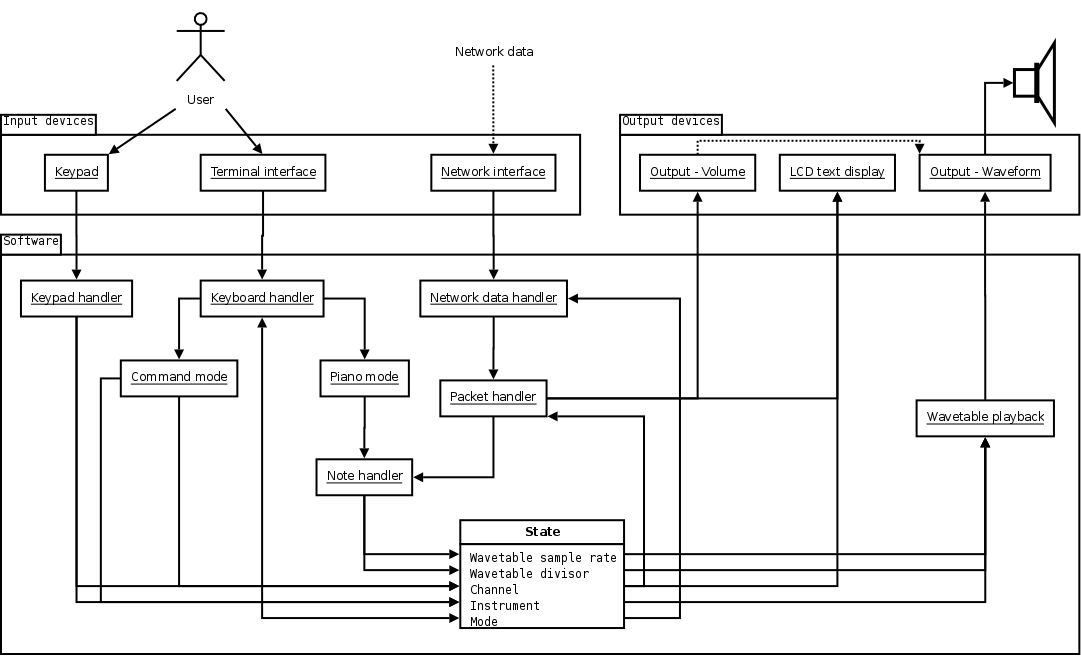
\includegraphics[totalheight=0.55\textheight,angle=90]{images/overview.png}
\caption{System overview}\label{fig:systemoverview}
\end{figure}
\end{nowordcount}

The diagram in Figure \ref{fig:systemoverview} shows the conceptual architecture of my system.  The 
basic idea is that various inputs are processed and in some way modify the state of the system, and 
this state in turn affects the operation of the continuously-running wave table playback.

The most important element of the system is the real-time conversion of network data to audio.  The 
network interface is a serial connection with a 19200bps baud rate.  Data arrives at a rate of one 
34-byte packet every 34ms.  The data format is sixteen pairs of bytes, each pair containing a MIDI 
note value and a volume level (both in the range 0--127), with each pair representing a channel 
between 0 and 15 (in order), and the packet is terminated with a null byte (00h) and a carriage 
return (0Dh).  The mapping of channel identifiers to instruments is shown in Table 
\ref{tab:channelids}.  For the ``Percussion'' channel, the volume level represents the particular 
percussion instrument to play rather than the volume at which to play it.

\begin{nowordcount}
\begin{table}[htbp]
\centering
\begin{tabular}[bp]{c l}
ID & Instrument \\
\hline
0 & Bass Guitar \\
1 & Cello \\
2 & Church Organ \\
3 & Piano \\
4 & Saxophone \\
5 & Melody \\
6 & Violin \\
7 & Trombone \\
8 & Trumpet \\
9 & French Horn \\
10 & Synth \\
11 & Electric Guitar \\
12 & Acoustic Guitar \\
13 & Flute \\
14 & Piccolo \\
15 & Percussion
\end{tabular}
\caption{Network data channels}\label{tab:channelids}
\end{table}
\end{nowordcount}

\subsection{Network}

% FIXME: contradiction with actual design?
The network handler deals with collecting data from the incoming bytes on the serial interface 
connected to the network and running the packet handler when the end of a packet is detected.  The 
carriage return is interpreted as the end of the packet, and the incoming bytes are counted and 
checked to detect and ignore incomplete packets.

When the end of a complete packet is detected, the packet handler is run.  The volume is converted 
from a 7-bit to 8-bit value and sent to the volume output, and also converted to hexadecimal and 
displayed on the LCD.  The MIDI note is used as the index in a lookup table for the PRT reload value 
and wave table divisor (see \ref{wavetables}), and also in another lookup table for a 4-character 
representation of the note which is shown on the LCD.

\subsection{Wave tables}
\label{wavetables}
% TODO: double check the maths!

In my design, all frequencies of the instruments are synthesised from the same wave table sample, 
therefore a way is needed to perform this frequency conversion.  A sample has two important 
interdependant properties --- the sample rate and the frequency.  When changing either of these 
properties, the following property holds:

\[\frac{F_{target}}{F_{source}} = \frac{R_{target}}{R_{source}}\]

In other words, if a particular note is recorded at a particular sample rate, then the difference of 
the frequency when played is proportional to the sample rate it is played at.  In this case, we are 
aiming to play a particular frequency, so the required sample rate can be calculated with:

\[R_{target} = \frac{F_{target} \times R_{source}}{F_{source}}\]

Unfortunately, at higher playback frequencies the necessary sample rate will be impractically high, 
so an additional way of changing the frequency is needed.  If for example only every other sample 
from the wave table is played, without changing the sample rate, this will double the frequency of 
the note being played, since the entire sample is being played twice as fast.  More generally, if a 
divisor $D$ is introduced, then $F_{target} = F_{source} \times D$.

To combine the two methods, $F_{target}$ can be replaced with $F_{target} \times D$.  With a little 
re-arrangement, the following equation can be obtained:

\[R_{target} \times D = \frac{F_{target} \times R_{source}}{F_{source}}\]

See \ref{notelookuptables} for how this conversion is implemented to generate the MIDI note lookup 
tables.
